\chapter{System Architecture}
\label{chp:architecture} 

The purpose of this thesis is to build an end-to-end system, to be able to transfer data all the way from sensors connected to a microcontroller to a server. This chapter will describe in detail how the different components of the system has been connected together, and how the different protocols has been configured to read and transfer data efficiently. 


\begin{figure}[ht]
    \centering
    \includegraphics[scale=0.7]{MasterArchitecture2.png}    
    \caption{System architecture}
    \label{fig:systemArchitecture}
\end{figure}

Figure \ref{fig:systemArchitecture} shows how the complete end-to-end system of this thesis is set up. In short terms, the \textit{Nordic Semiconductor nRF52} is connected to a  \textit{Raspberry Pi 3} using \gls{6lowpan} and \gls{ble}. This means that they are able to communicate using \gls{ipv6} addresses, even though the nRF52 only has a bluetooth antenna built in, as shown in figure \ref{fig:nrf52chipDetail}. The limitations of \gls{ble} means that the nRF52 can only connect to \textit{one} device at the time. Several of these put together are therefore forming a \textit{star network} using the \textit{Raspberry Pi} as a central point of connection. Computations can now either be done in the end nodes at the \textit{nRF52s}, at the \textit{Raspberry Pi}, or forwarded to a web server or another computer with more computational power. Data can also be displayed directly to a web page from the \textit{Raspberry Pi}. 
 
%\newpage

There are in general three main limitations in a network such as this:

\renewcommand{\labelitemi}{$\textasteriskcentered$}
\begin{itemize}
  \item Computational power in the different nodes
  \item Battery capacity of the end nodes
  \item Network limitations between the nodes
\end{itemize}

A central part of the testing in this thesis will be to test the different limitations, and to understand the pros and cons of doing computations in end nodes, compared to transferring information to a server with \textit{much} more computational power. Power usage is very often closely related to computational power, and will also be a central factor. The next section will contain a walk-through of the system, from the smallest to the biggest component, to explain their computational and power capabilities, and how they can communicate efficiently. 

Computational power is closely related to power usage. The nRF52 microcontroller is battery powered using a small \textit{3V Lithium CR 2032} battery. Given this limitation the computational power will be limited as well. The optimal solutions therefore seems to handle as little data as possible here. 


\section{Connecting Raspberry Pi and nRF52}


%As a microcontroller the nRF52 works good in this network, both as a low-power and powerful device. 

To set up the communication between a Raspberry Pi and the nRF52, the two code examples TWI and Observable server from Nordic Semiconductor was used as a starting point for coding on the nRF52. It was however quite tricky to set connect these two together the first time. The following recipe is what worked best. 

Install an \gls{os} on the Raspberry Pi that has a Linux kernel version later than 3.18. On \textit{Raspbian} version 3.18 is the only stable (Note: Jan. 2016), but \textit{Ubuntu Mate} is stable in version 4.15. \textit{Ubuntu Mate} was therefore chosen as the best and most stable \gls{os}. When this is done a resizing of the file system is needed to use all the capacity of the memory card. This is not necessary, but recommended to be able to use more than 4GB of the memory card. To resize, run the following commands

\begin{verbatim}
sudo fdisk /dev/mmcblk0
\end{verbatim}

Delete partition (d,2), and run the following after a reboot

\begin{verbatim}
sudo resize2fs /dev/mmcblk0p2
\end{verbatim}

To use \gls{ble}, install Bluez and radvd using \textit{apt-get} in a \textit{Unix terminal}:

\begin{verbatim}
apt-get install radvd wireshark bluez
apt-get upgrade
apt-get update
\end{verbatim}
%\end{lstlisting}

To activate \gls{ipv6} forwarding, uncomment the following line (remove "\#") in the file \textit{etc/sysctl.conf}

\begin{verbatim}
net.ipv6.conf.all.forwarding=1
\end{verbatim}

Add the \textit{bt0 interface} in \textit{radvd.conf}:

\begin{verbatim}
touch /etc/radvd.conf
pico /etc/radvd.conf
\end{verbatim} 

Write in the bt0 interface

\begin{verbatim}
interface bt0
{
    AdvSendAdvert on;
    prefix 2001::/64
    {
        AdvOnLink off;
        AdvAutonomous on;
        AdvRouterAddr on;
    };
};
\end{verbatim} 

To mount the modules \textit{bluetooth\_6lowpan, 6lowpan and radvd}, add the following to \textit{/etc/modules}. 

\begin{verbatim}
bluetooth_6lowpan
6lowpan
radvd
\end{verbatim}

It is now possible to use the \textit{hcitool} command. 

\begin{verbatim}
hcitool lescan
\end{verbatim}

This command will scan for \gls{ble} devices nearby, and find the bluetooth address, for instance \textit{0211:22FF:FE33:4455}. The normal procedure in this case would be to run the following command: 

\begin{verbatim}
echo 1 > /sys/kernel/debug/bluetooth/6lowpan_enable
hcitool lecc 0211:22FF:FE33:4455
service radvd restart
\end{verbatim}

This command never established a stable connection in this system. It was not possible to test the connection, and each connected device became automatically disconnected after about 15 seconds. The reason for this was never found. Instead it was possible to not use \textit{hcitool} for this part, and the following commands worked fine:

\begin{verbatim}
echo 1 > /sys/kernel/debug/bluetooth/6lowpan_enable
echo "connect 0211:22FF:FE33:4455 1" > /sys/kernel/
debug/bluetooth/6lowpan_control
service radvd restart
\end{verbatim} 
\todo{FIX verbatim new line? }

The command \textit{hcitool con} shows the connected \gls{ble} devices. If the device is connected, the connection can be tested by typing:

\begin{verbatim}
ping6 2001::0211:22FF:FE33:4455
\end{verbatim}


Using the basic examples provided by Nordic Semiconductor described in chapter \ref{chp:architecture}.3, it was now possible to send messages both using \gls{coap} \gls{con} and \gls{non}.  


\section{Connecting nRF52 and ADXL345}

\todo{Can possibly write much more here, code samples in appendix, things that needed to be changed and so on}

The ADXL345 Accelerometer used was connected using \gls{i2c}, which is quite straight forward using the nRF52. Connection scheme is as follows (nRF52 -> ADXL345): 

\begin{itemize}
  \item 5V -- VIN		\tab  	\textit{Power source, \textbf{\textcolor{green}{green cable}} in Figure \ref{fig:nrf-adxl345}}
  \item GND -- GND 		\tab 	\textit{Ground, \textbf{\textcolor{red}{red cable}} in Figure \ref{fig:nrf-adxl345}}
  \item P0.27 -- SDA	\tab	\textit{\gls{i2c} Serial Data Line, \textbf{\textcolor{orange}{orange cable}} in Figure \ref{fig:nrf-adxl345}}
  \item P0.26 -- SCL	\tab 	\textit{\gls{i2c} Serial Clock Line, \textbf{\textcolor{brown}{brown cable}} in Figure \ref{fig:nrf-adxl345}}
\end{itemize} 

%\begin{figure}[ht]
%    \centering
%    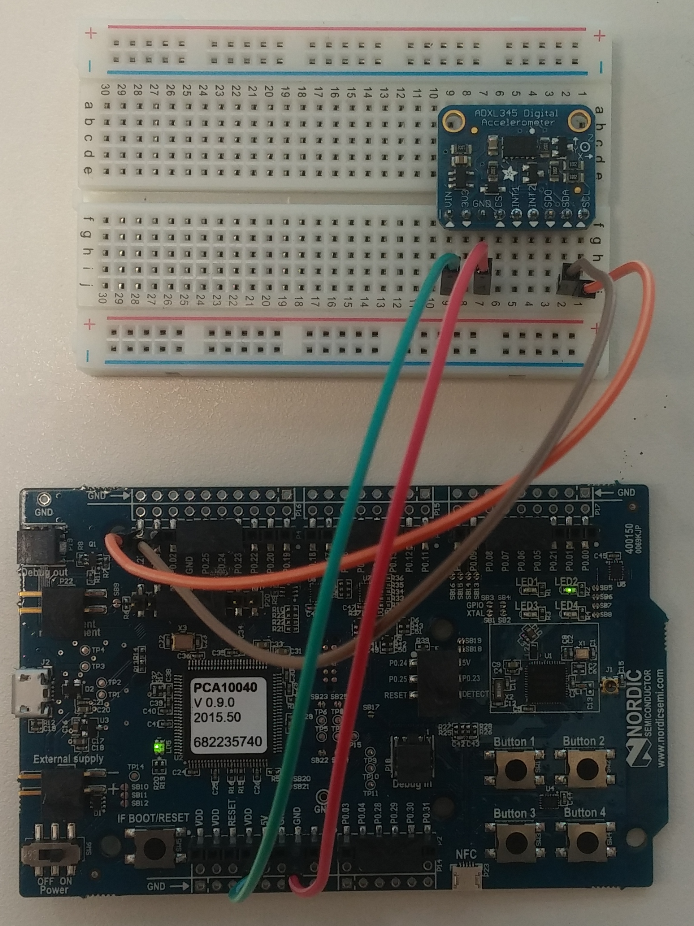
\includegraphics[scale=0.35]{nrf-adxl.png}    
%    \caption{Connected nRF52 -- ADXL345}
%    \label{fig:nrf-adxl345}
%\end{figure}


\begin{figure}[ht]
    \centering
    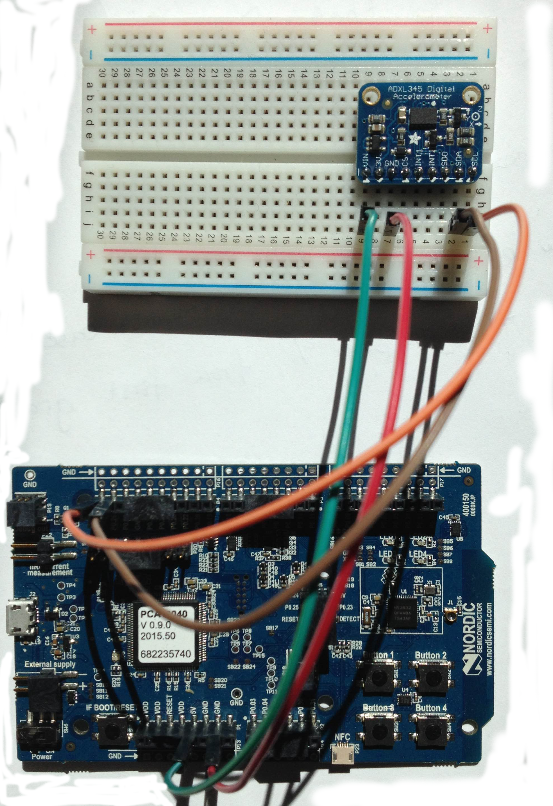
\includegraphics[width=0.6\textwidth]{connectionADXL-nrf3.png}    
    \caption{Connected nRF52 -- ADXL345 2}
    \label{fig:nrf-adxl345}
\end{figure}

After this is done it is possible to write to and read from the registers of the accelerometer over the two SDA and SCL cables. 


\subsection{Connection challenges}

Following instructions from a representative from Nordic Semiconductor, the bt0 interface was set up using the recommended \gls{ipv6} prefix: \textit{2001:bt8::1/64} in in the file \textit{etc/sysctrl.conf}, and after that trying to connect and test the connected devices using addresses on the form: 

\begin{verbatim}
ping6 2001:bt8::0211:22FF:FE33:4455
\end{verbatim}

This turned out not to work on the \gls{ipv6} network used on \gls{ntnu}, where the standard prefix is \textit{2001::1/64}, without the \textit{db8}. Both solutions should however work in other \gls{ipv6} networks. 

\subsection{bt8}

\todo{Descibe bt8-problem and devzone.nordicsemi.com and infocenter.nordicsemi.com}

\todo{Describe why I dropped the accelerometer}



\section{Nordic Semiconductor example code}

Nordic Semiconductor has provided several examples along with the nRF52-DK documentation, that can be used as a starting point when programming applications to the device. These files are written in the programming language \textit{C}. 

\subsection{\gls{coap}}

As a first step, the nRF52 needed to communicate with the Raspberry Pi. As explained in section 2.6, a good starting point for this is to use the \gls{coap} trasnport protocol, and the example of the use of this on the device. The \textit{CoAP Server} and \textit{CoAP Observer} was loaded into two different nRF52 devices, and both of them connected to the Raspberry Pi. Now \gls{radvd} had to be activated on the Pi, to be able to use this as a \textit{forwarding server}. 

\begin{figure}[ht]
    \centering
    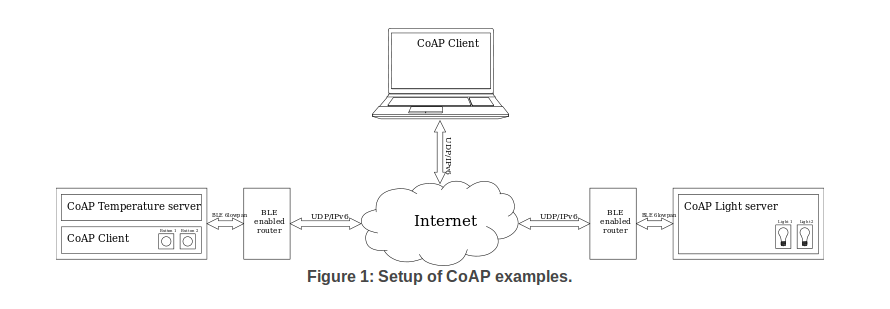
\includegraphics[scale=0.47]{CoAPExample.png}    
    \caption{CoAP Client-Server communication example}
    \label{fig:CoAPexample1}
\end{figure}
\todo{Remove "Figure 1" from image}

Figure \ref{fig:CoAPexample1} shows the initial CoAP example, by using two nRF52 devices, \gls{ble} over \gls{6lowpan} and a \gls{ble} enabled router (Raspberry Pi) on both ends in this case. As the figure \ref{fig:CoAPexample1} shows, the code example for the \gls{coap} client includes two different cases: 

\begin{itemize}
  \item In the fist case the \gls{coap} client acts as a client requesting services from the \gls{coap} server. Button 1 and 2 will control light 1 and 2 on the nRF52 server, which will send a conformation back if the light was changed or if something went wrong.
  \item In the second case the \gls{coap} server is excluded, but the \gls{coap} client works as a server that can handle requests from the router. In this case it is possible to use \textit{Copper} in a \textit{Firefox browser} on the Raspberry Pi to act as a client to request values from a simulated temperature sensor on the server. The server will  then send the current simulated temperature back, or tell if something went wrong. 
\end{itemize} 

Figure \ref{fig:CoAPexample1} shows the capture of packets using Wireshark. 

\begin{figure}[ht]
    \centering
    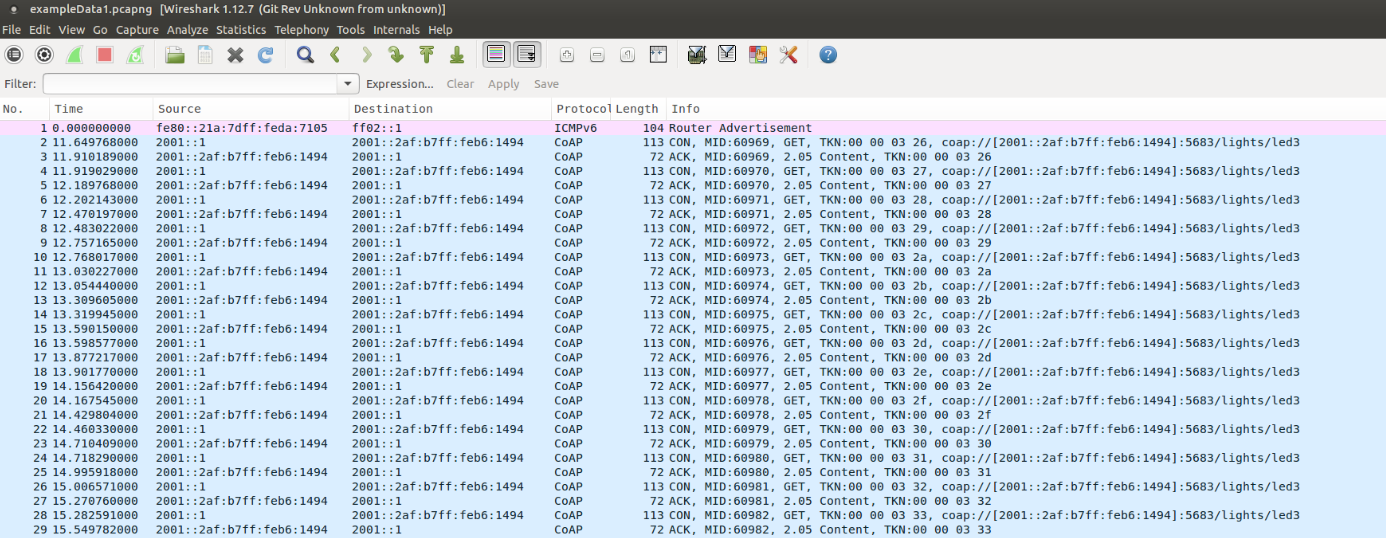
\includegraphics[scale=0.27]{CoapEx1captureCropped2.png}    
    \caption{CoAP Client-Server example Wireshark capture}
    \label{fig:CoAPexample2}
\end{figure}


This gives us the sequence diagram shown in Figure \ref{fig:seq1}. 

\begin{figure}[ht]
    \centering
    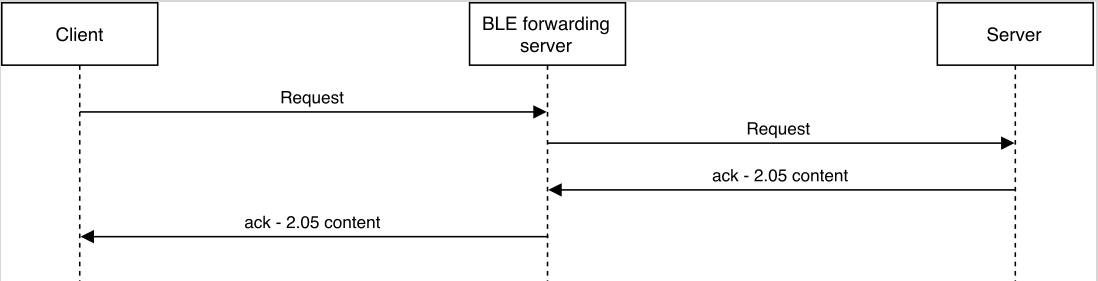
\includegraphics[scale=0.27]{seq1.png}    
    \caption{Sequence diagram CoAP Client-Server example}
    \label{fig:seq1}
\end{figure}

\todo{Create new sequence diagram}

This works fine, and by writing a Python script running on the \textit{Raspberry Pi} it is possible to request data by \textit{GET messages} as soon as the \textit{nRF52} is ready. However, as shown in figure \ref{fig:pingComparison} and figure \ref{fig:ping2}, the network transfer rate can vary a lot. The limitations in \gls{ble} and \gls{6lowpan} makes this much slower than a standard \gls{ipv6} connection, and the \textit{ping} \gls{rtt} varies from 100 ms all the way up to over 600 ms. As a comparison, to \textit{ping google.com} from the same Raspberry Pi using \gls{ipv6} takes on average 15 ms. A comparison of this is shown in figure \ref{fig:pingComparison}. This is therefore a clear limitation of sending rate in the system. Because of this, the maximum transfer rate achieved in the system using the standard \gls{coap} server example is one message every 200 ms. 

Using the standard \gls{coap}, described as \textit{CoAP CON} in this thesis, messages are sent with a "\gls{tcp} mindset". This means that every message sent by the client must receive an \gls {ack}. This is very stable, and ensures that every message gets to its destination, but it requires a lot of unnecessary computational power in the leaf node in systems where the importance of each message is not that high. The system is meant to be used with tools for analysing, and it is not essential that data needs to get to its destination right away. In these cases there is another alternative, known in this thesis as \textit{CoAP NON}. This is more like a "\textit{gls{udp} mindset}", where each packet does \textit{not} need an \gls{ack}. This halves the number of packages sent, saves a lot of the network as well as actions needed to be done by the nRF52 where power consumption is a huge issue. Therefore the \textit{\gls{coap} Observable} function looked very interesting, and will therefore be directly compared to \textit{standard gls{coap}} later in this thesis.   

%To improve this, the best solution is to either 

%This works fine, but in the case of the system built in this thesis there is no need to receive a confirmation for every single message.  It therefore makes sense to send messages in an \textit{\gls{udp} fashion}, where packages are being sent right away without acknowledgement. .   

\subsection{Observable \gls{coap}}

In the given Nordic example of a \gls{coap} observable server, the problem of unnecessary packets being sent can be resolved. Using this it is easy to set up a server that can be observed by either a nRF52 client or a \gls{ble} forwarding server. The observable end point sends a \textit{CON-ACK request} in a given time interval to assure that the observing client is still there. As long as this message is being responded the server will continue to send data without any requirements of an \gls{ack}. 

\begin{figure}[ht]
    \centering
    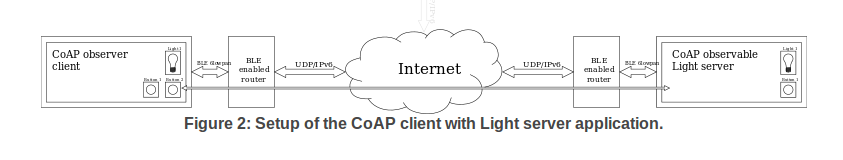
\includegraphics[scale=0.47]{CoAPObservalbFigure2.png}    
    \caption{CoAP Observable Server example}
    \label{fig:CoAPexample2}
\end{figure}
\todo{Remove "Figure 1" from image}



\todo{Create new sequence diagram for Observable as well}


\section{Getting acceleration values}

As soon as the sending of values is being handled in a good way, the next step is to read acceleration values from the ADXL345 accelerometer, which is connected to the NRF52 using the \gls{i2c} interface. 

Acceleration values can only be read from the ADXL345 if this has been correctly initialized at compile time. In order to do this, code to write to and read from the registers had to be added. The initializing process is described in the accelerometer data sheet \cite{adxlDataSheet}. In short, registers for \textit{data format control, initial power saving, interrupt enable control} and \textit{the offset of each axis} has to be written to in that order before the acceleration value from the different axes can be read.  

In the solution proposed in this thesis the acceleration values are being read as often as possible, limited by the processing power of the nRF52, and then stores in a simple dynamical char array before being sent and reset after one second. This turned out to be very time consuming and hard to solve in a good way, both because of problems with initializing the accelerometer correctly and making the nRF52 read and store the values fast enough to get proper data. The ideal solution would be to read at least 1000 values every second, to get a good starting point before analysing values. Neither the nRF52 or the ADXL345 turns out to be fast enough to do this in the implemented solution.  To not loose too much time on hardware problems, it was decided to focus more on analysing the data sent over the network communication with random generated data. 

Since the network connection between the nRF52 and Raspberry Pi was already stable, it was easy to generate random values of fixed length to send on the nRF52, and do measurements to calculate the optimal throughput between these two. The next chapter will therefore describe the data analysis of the data sent through this network in detail, and how to optimize the percentage of usable data being transported.  

\todo{Describe why not to gather acceleration values in this project}


\section{From Raspberry Pi to Network Computer or Server}

When running the Unix based \gls{os} Ubuntu Mate, the raspberry Pi can be used more or less as a regular computer. This has a pre-installed version of the most basic programs needed, for instance \textit{Mozilla Firefox Browser}, \textit{Pluma text editor} and \textit{Unix terminal}. This means that the user has several options on how to process data on this device: 

\begin{itemize}
  \item No computation: All data arrives as useful data, and can be posted directly to a web page or a server for storage
  \item No computation: Forward all data directly to a computer with more computational power
  \item Some computation: Analyse the data to find data that is not relevant to filter out
  \item Full computation: Do a full analyse of the data. The results can then be posted directly to a server or displayed on a web page. 
\end{itemize}

Which of these four options that is most relevant depends on the data, and how computational power is needed. It is possible to run the Raspberry Pi from a power bank, but this has not been tested in this project. When set up without a battery as power source, the Pi is the first node that could possibly do computations without having to take power limitations as a great concern. The main limitation is therefore computational power, while the main limitation may be battery power on the nRF52. It therefore makes sense to do some easy computation on this device. For instance, if this network is being used to measure vibrations, it is reasonable to assume about 1000 acceleration values every second, which represents a measuring rate of 1 kHz. It would then be perfectly reasonable to assume that the Pi could go through these values, and calculate whether or not the current acceleration value has breached a given threshold. This result can then be displayed directly on a web page or a connected monitor from the Pi. If however the system is to calculate \textit{patterns} in the acceleration values several values needs to be compared together. The need of complex algorithms to find these patterns is expected, before the results can be displayed. In this case it is reasonable to assume that the Pi would need additional computational power. The Pi can then be set up as a forwarding device, that forward data directly to a computer with more computational power. 

